\subsection{Adaptive Parallel Plan Management Algorithm}
\label{subsec:plan_management-adaptive_parallel_plan_manager}
In real cooperative operations, a serialized execution is not enough. The most natural way to interact is, in fact, parallelizing the agents' actions when this is possible. We created a new plan management algorithm to address this issue. We will illustrate its main points.

\subsubsection{Plan Preprocessing}
To start, we pre-process the plan streams produced by the Task Planner. Normally, the plan streams only include low level actions. We need to  modify the humans' plan streams to account for high-level tasks to be monitored. In this new plan, we may substitute groups of nodes with one of their ancestors, when the knowledge level of the human of the ancestor node's task is competent enough, and we want to give him flexibility. This new node will only have casual links in its plan stream, imagining that the human will account on its own to coordinate with other agents. If another agent had a casual link on a removed node, we remove this casual link, but remember this information, as we will account for it in the plan management algorithm.

We will, so, analyze each node $n$:
\begin{itemize}
\item We look in the HTN tree for the oldest ancestor of $n$, that we call $a$, where $kn(a) \geq intermediate$. Note that this node must exist, as $n$ is a leaf (since the plan streams are composed only by leaves of the HTN tree), and we consider leaves as common actions, as explained in section \ref{sec:plan_management-human_knowledge}.

\item If $a$ is different than $n$, let $[n_1..n_m]$ be the list of children of $a$. We substite this list, in the plan stream, with $a$. We set the casual links of $a$ with the predecessor of $n_1$ in the stream and the successor of $n_m$ in the stream (if they exit).
\item For each casual link $l$ starting from any node $m$, where $m$ is a node in a different agent's plan stream, we erase $l$, but record this information in a new flag associated to the node, that we call \textit{had\_casual\_link}.
\end{itemize}


\subsubsection{Algorithm}
After pre-processing the plan streams, the plan manager can start executing the current plan. Each stream will be executed in its own thread. First, we will start explanining the robot's algorithm, which we divide in three blocks: a \textit{control} block, which leads the flow of the program, an \textit{action} block, which controls the execution of actions, and an \textit{explain user} block, which manages eventual explanations to users. We will now details each of these block, starting with the \textit{control} block algorithm, shown in figure \ref{fig:plan_management-manage_plan_leader_control_block}:
\begin{itemize}
\item The plan management algorithm needs to execute $n$ robot actions.
\item If the stream receives an explanation request from the Plan Manager of another agent, the algorithm proceeds in the \textit{explain user} block.
\item If the current plan is not completed, and the algorithm did not receive a failure report from another Plan Manager, the system will wait for the casual links of the current action, using the \textit{waitCasualLink} procedure, which was already explained in subsection \ref{subsec:plan_management-robot_not_leader_manager}.
\item If the system receives an error from another Plan Manager, it will fail, prompting a replan. Otherwise, when the casual links are all satisfied, it will transition to the \textit{action} block.
\item If the plan of the robot is completed, but there are still some users acting, the robot will wait for them to finish their plan, limiting itself to provide explanations, if needed.
\item The Plan Manager terminates successfully when all the agents have completed their plans.
\end{itemize}


\begin{figure}[ht!]
 \centering
 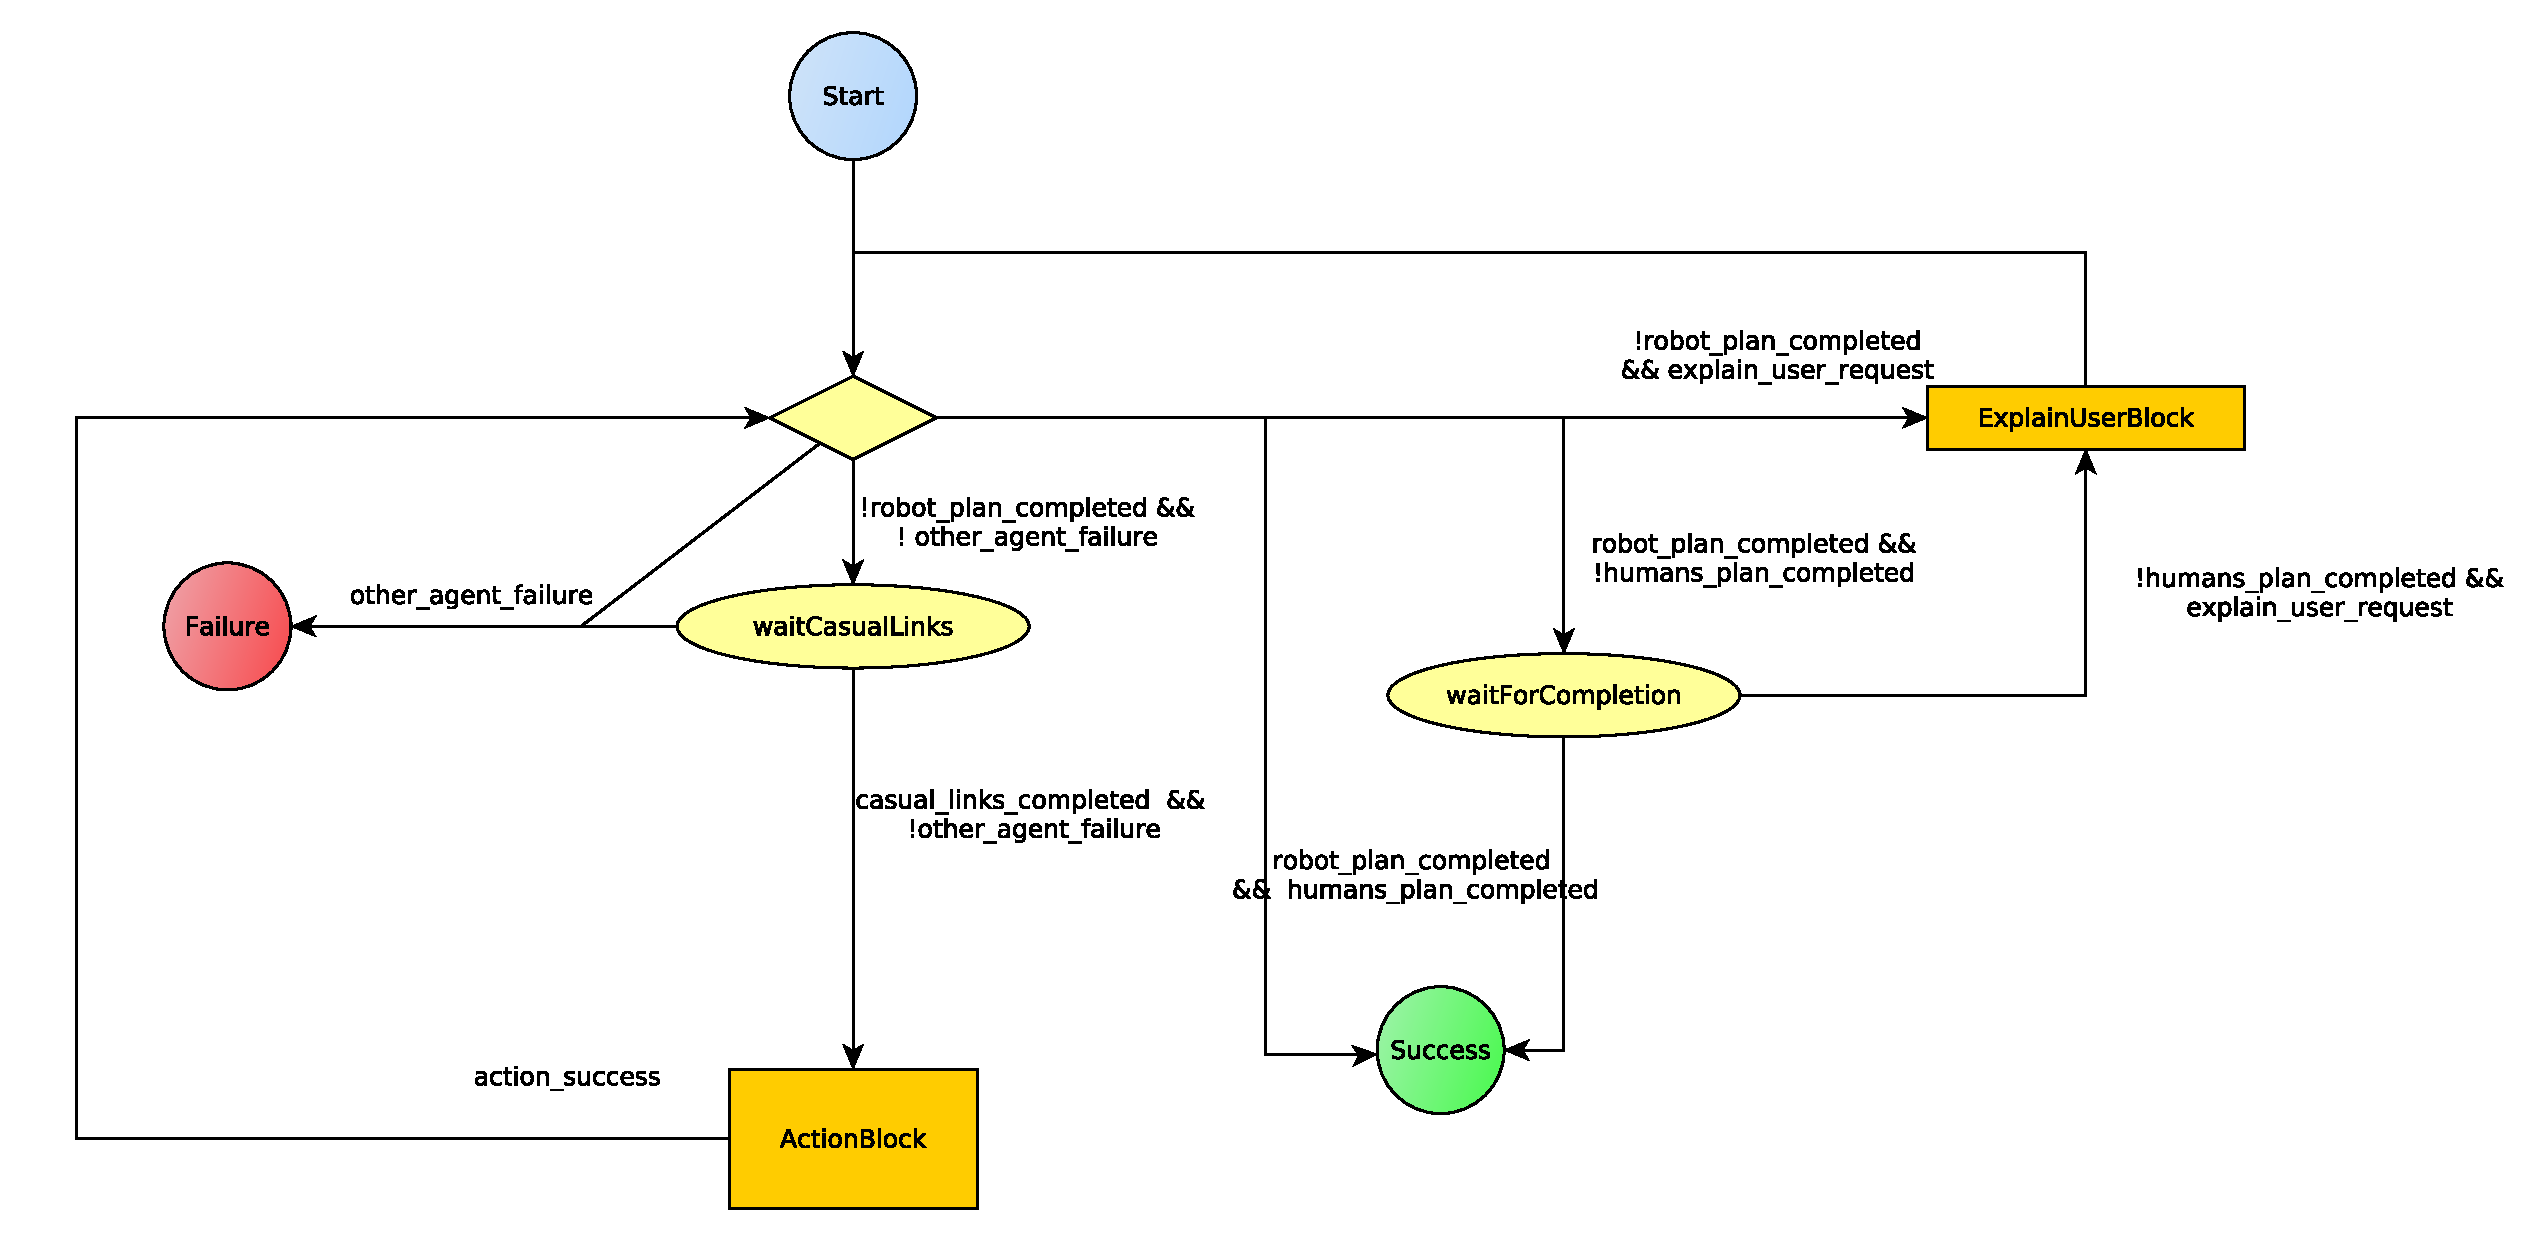
\includegraphics[scale=0.45]{img/plan_management/manage_plan_leader_control_block.pdf}
 \caption[The control block of the parallel plan management algorithm]{The control block of the parallel plan management algorithm used when the current modality is \textit{robot leader}. The symbols used are the same as in figure \ref{fig:plan_management-manage_plan_not_leader}, with the exception of yellow rectangles, which represent other blocks in the algorithm.}
 \label{fig:plan_management-manage_plan_leader_control_block}
 \end{figure}


We continue by explaining the \textit{action} block algorithm, shown in figure \ref{fig:plan_management-manage_plan_leader_action_block}.
\begin{itemize}
\item At the start of this block, the robot will analyze the current action to understand if it needs to verbalize it to users. In order to do so, it will look for the ancestors of the current node in the tree structure, using the same idea shown in the sequential plan management algorithm (lines ~\ref{alg:onlyRobotStart}-~\ref{alg:onlyRobotEnd}). The system will record which tasks have been explained, in order to avoid re-explaining the same task.
\item If the robot should explain some of his actions, it will transition to the \textit{explainAction} function. This function will verbalize the tasks, with the same reasoning shown in the sequential plan manager, if there are users in the same area as the robot.
\item Since the human might take actions that diverge from the robot's plan, the current action might not be executable. Imagine, for example, the case where the robot's current action is to take an object from a table, but that object is not there. There are two possibilities in this case. 1) There was a casual link $(a_h,a_n)$ where $a_h$ is an action that had to be performed by a human, and $a_n$ is the current action. The robot in this case has no way to know if the human has not yet performed the action, or if it will not perform it because he is following a different plan from the one it computed. 2) The human is following a different strategy, making $a_n$ not executable at the moment. For example, the human has taken an object needed by the robot. In this situation, the robot will wait from a predefined time for the action to become executable. If the action does not become executable in this time, the algorithm fails, prompting a replan.
\item If the action is executable but the \textit{had\_casual\_link} flag for $a_n$ is set, the robot will ask the human for permission to perform the action. In fact, we might find situations where the human had to use a shared resource $r$ linked to $a_n$ in the original plan, like an object. The robot can not know if the human is using a different strategy, where he does not need $r$, if he has already finished using it, or if he still needs it. Our solution to this problem is asking him for permission, which is done in the \textit{askPermission} procedure. 
\item If the action is executable, and the \textit{had\_casual\_link} flag is not set, or the robot had permission from the user, the system invokes the \textit{executeAction} procedure, which will go back to the control block in case of success, or return a failure in case of errors. 
\end{itemize}


\begin{figure}[ht!]
 \centering
 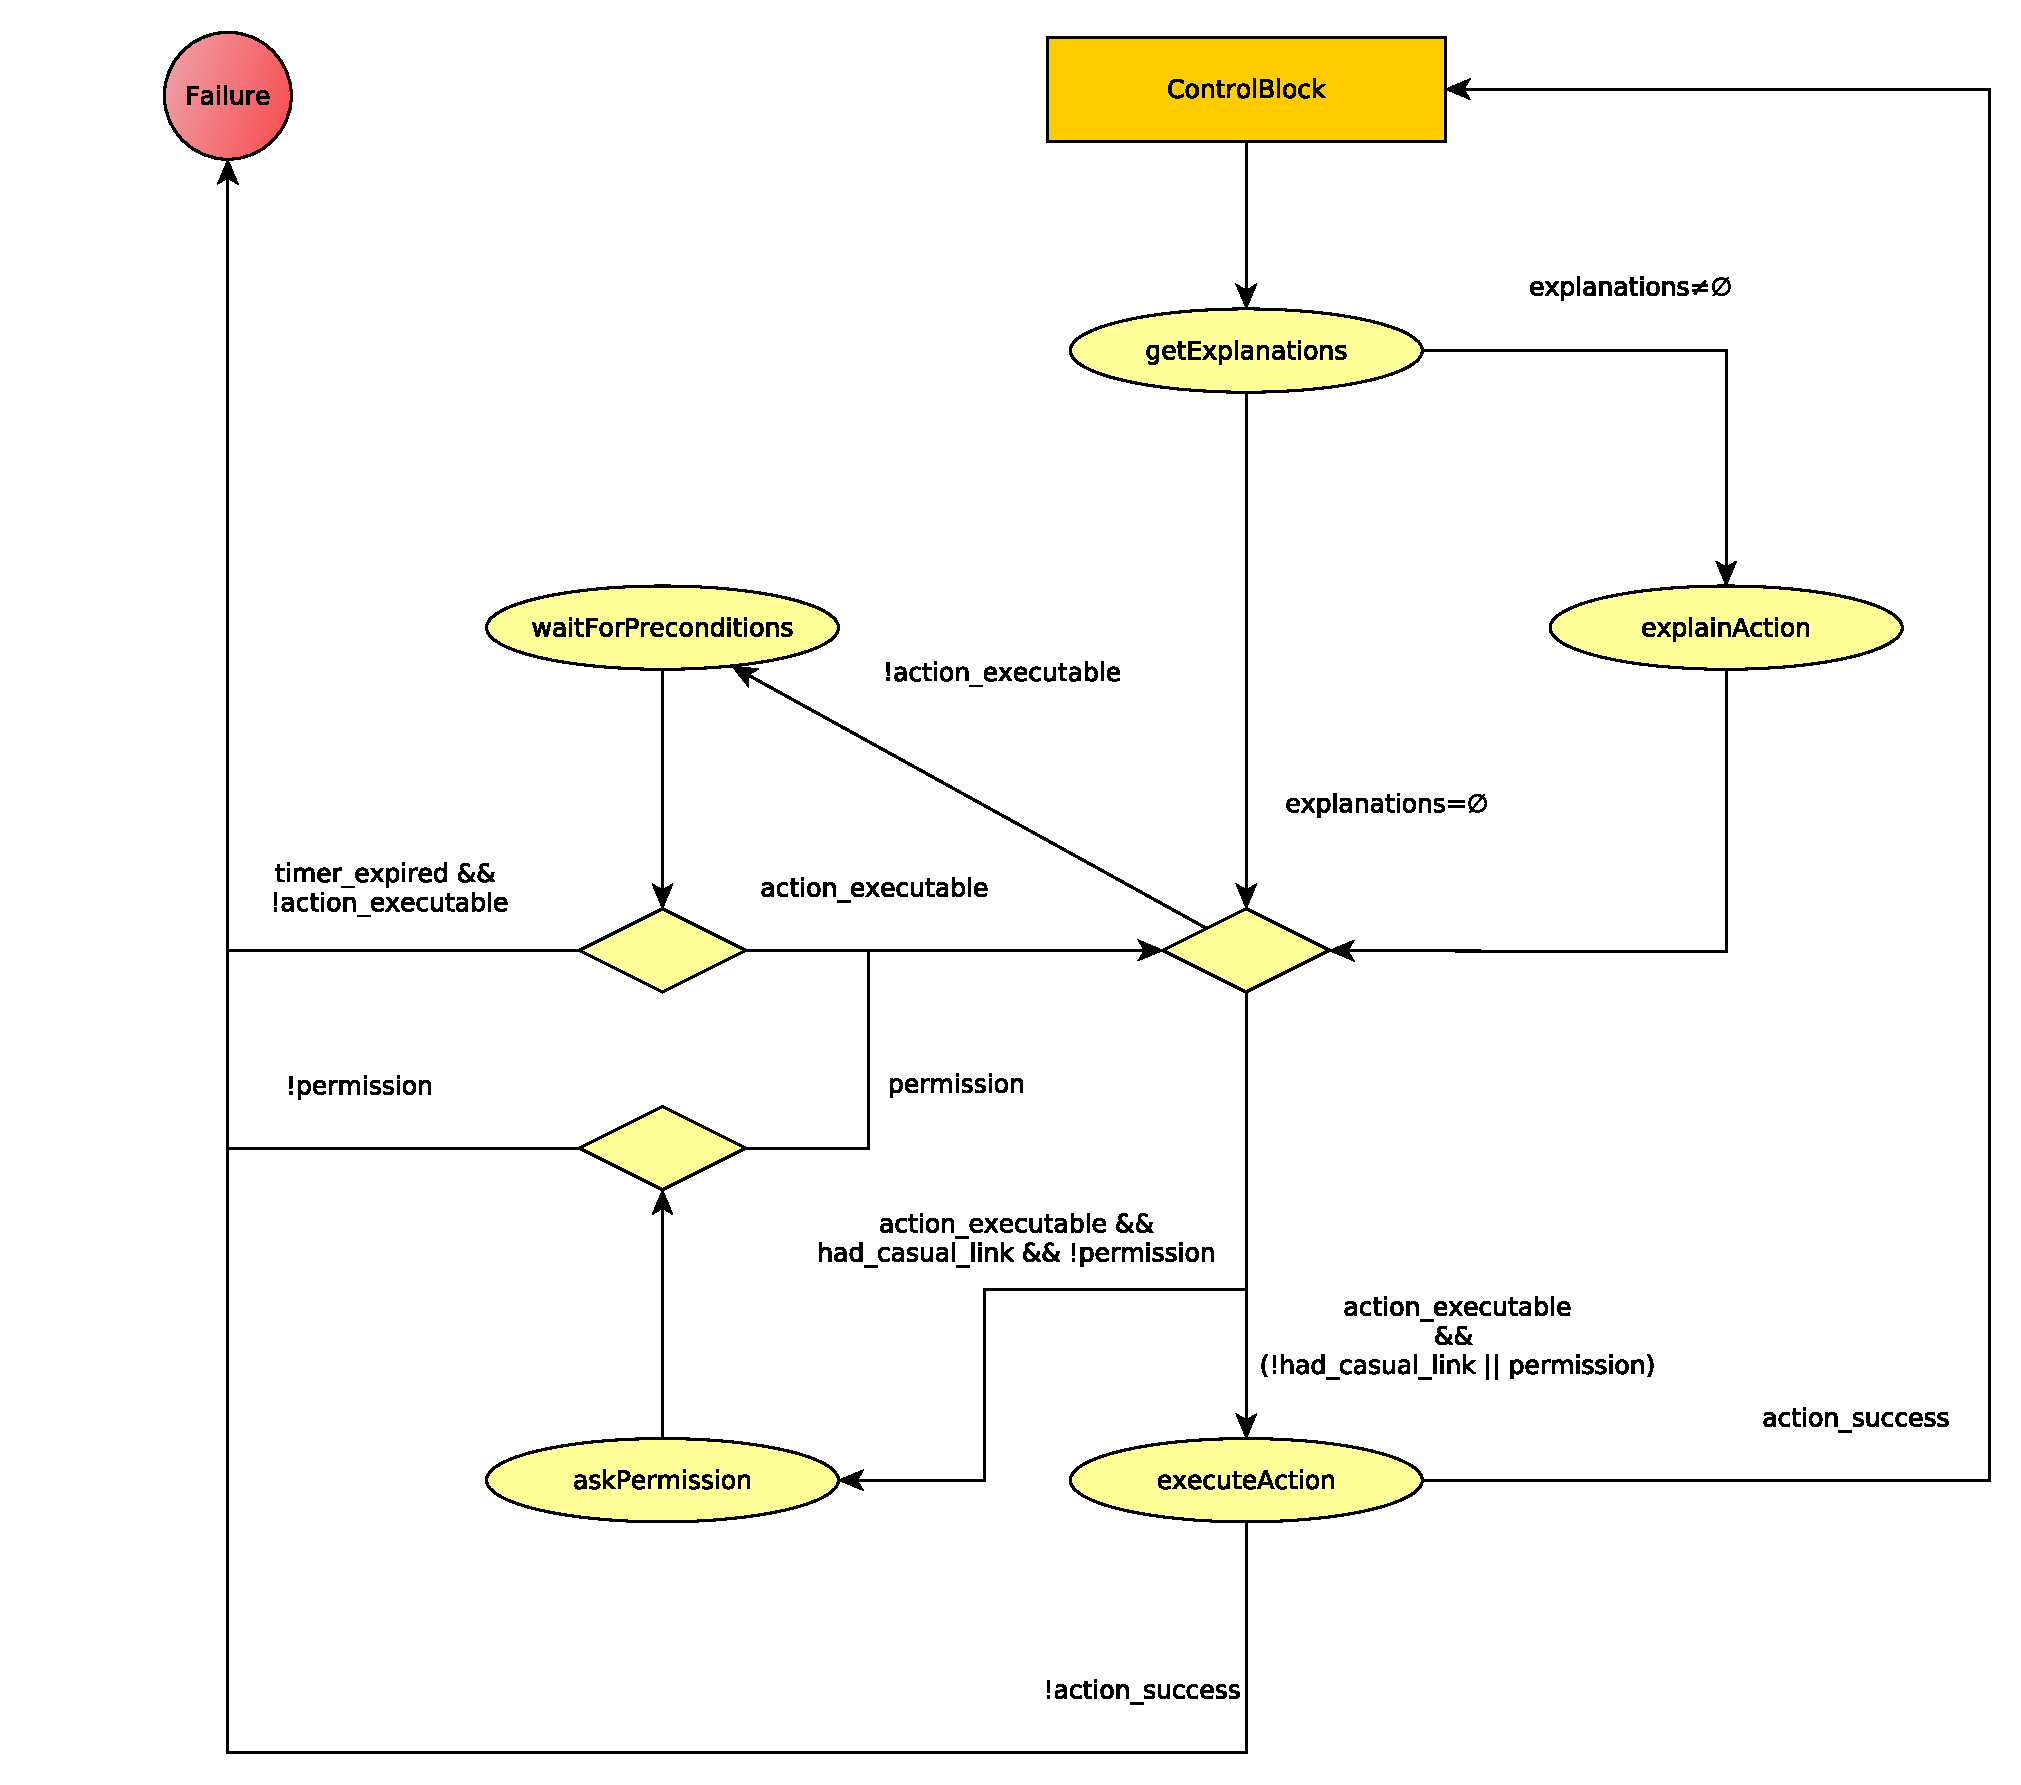
\includegraphics[scale=0.45]{img/plan_management/manage_plan_leader_action_block.pdf}
 \caption[The action block of the parallel plan management algorithm]{The action block of the parallel plan management algorithm used when the current modality is \textit{robot leader}. The symbols used are the same as in figure \ref{fig:plan_management-manage_plan_leader_control_block}. The algorithm starts from the ControlBlock node.}
 \label{fig:plan_management-manage_plan_leader_action_block}
 \end{figure}


Finally, we show the \textit{explain user} block algorithm, shown in figure \ref{fig:plan_management-manage_plan_leader_explain_block}.
\begin{itemize}
\item This block is invoked when the robot's Plan Manager received an explanation request from the Plan Manager of another agent.
\item To start, if the user is in a different location, the robot will move toward him.
\item At this point, if there are no errors, the robot will invoke the $explainUser$ procedure, which might explain him the task, or propose an explanation first, as explained in the sequential plan manager (lines~\ref{alg:newStart}-~\ref{alg:beginnerEnd}). 
\item If the robot changed his position, and his next action in the plan stream is not a $moveTo$ action, which would make it change location, the robot will go back to his previous location.
\item If there is an error during any of these operations, the system will look for a new plan.
\end{itemize}


\begin{figure}[ht!]
 \centering
 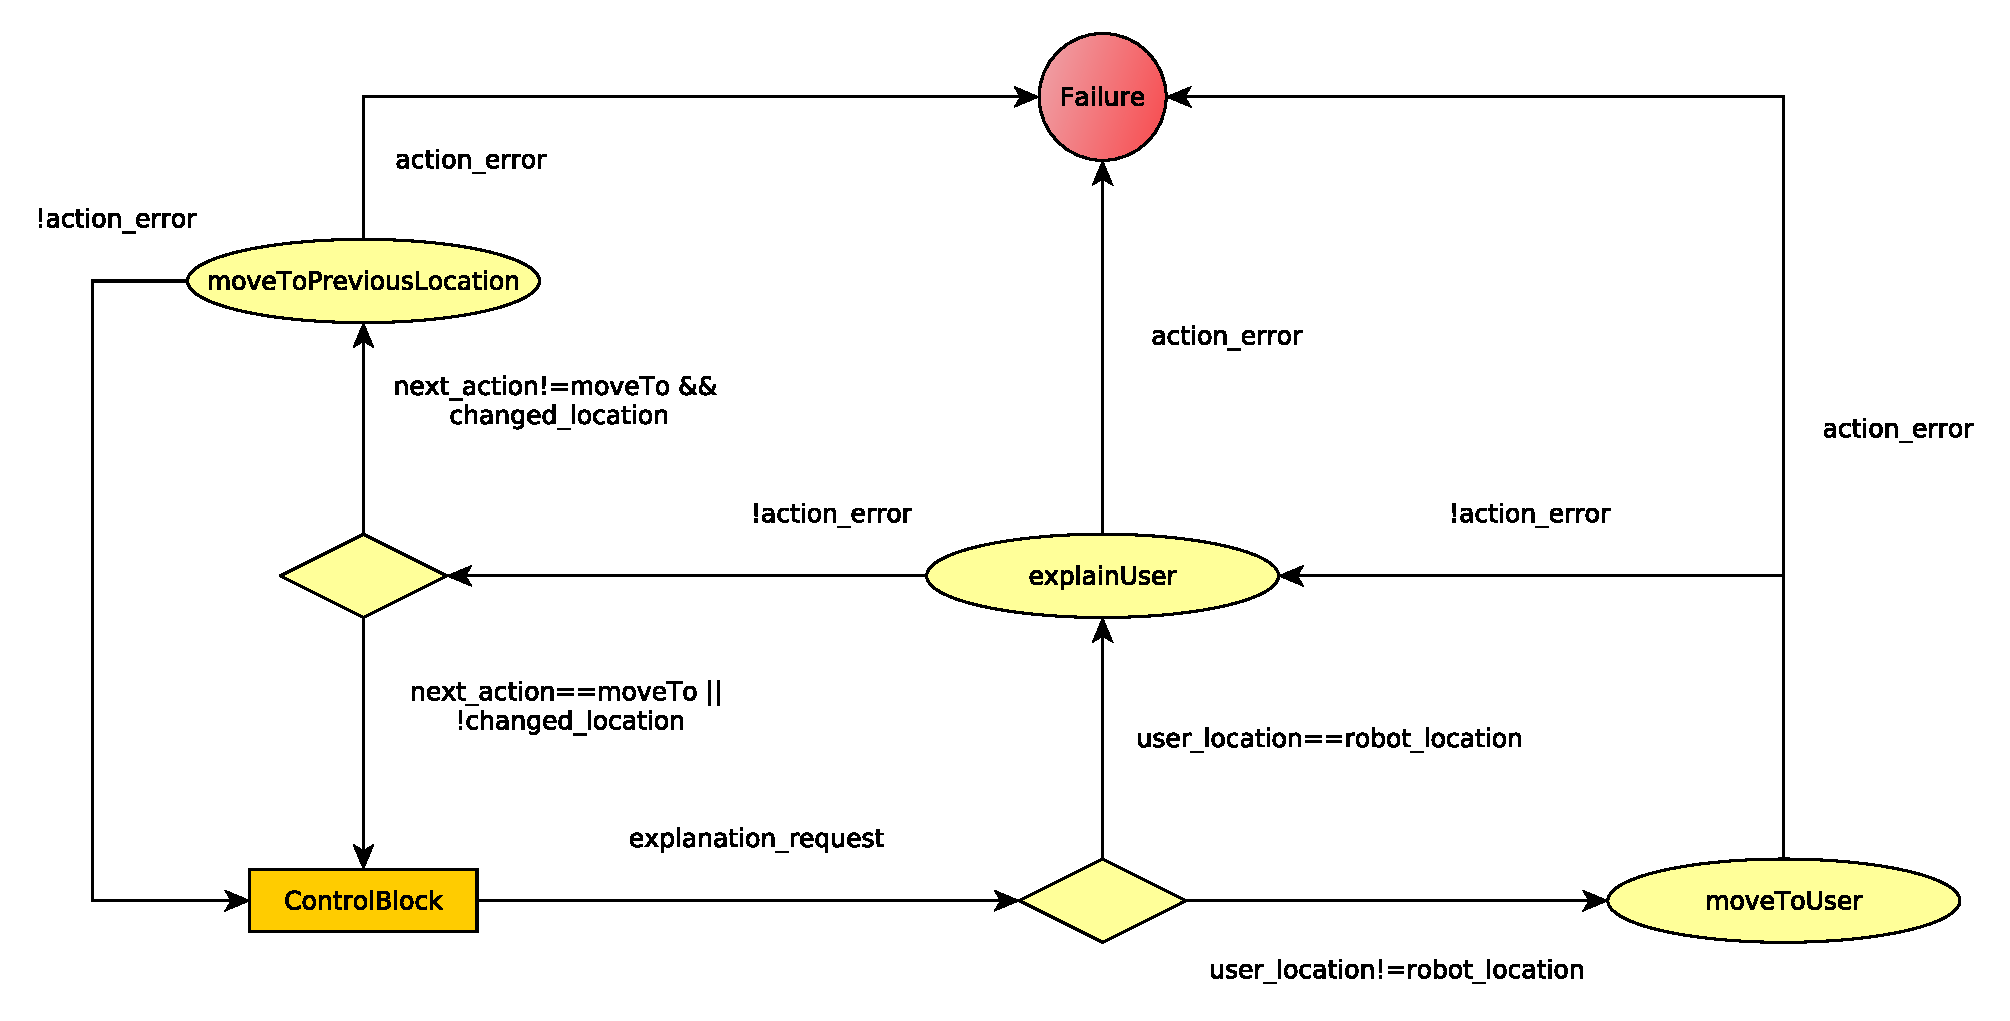
\includegraphics[scale=0.5]{img/plan_management/manage_plan_leader_explanation_block.pdf}
 \caption[The explain block of the parallel plan management algorithm]{The explain block of the parallel plan management algorithm used when the current modality is \textit{robot leader}. The symbols used are the same as in figure \ref{fig:plan_management-manage_plan_leader_control_block}. The algorithm starts from the ControlBlock node.}
 \label{fig:plan_management-manage_plan_leader_explain_block}
 \end{figure}


Now, we will explain the user plan management algorithm, shown in figure \ref{fig:plan_management-manage_plan_leader_humans}
\begin{itemize}
\item This algorithm is, in fact, very similar to the Plan Manager for the other two planning modalities, previously explained in section \ref{subsec:plan_management-robot_not_leader_manager}. The difference lies in the \textit{getExplanations} and \textit{requestExplanations} procedures.
\item The getExplanations procedure is used to decide if the robot should explain the current task of the human, propose an explanation, or simply monitor. This is done analyzing the ancestors of the node, with a similar process to the sequential algorithm (lines~\ref{alg:newStart}-~\ref{alg:beginnerEnd}).
\item If the current task should be explained, the system will send a request to the robot's plan management stream, using the \textit{requestExplanation} procedure. The system will then wait for the end of the robot's explanations or for an error.
\item If there are no errors the system will start monitoring the current task.
\item The process is repeated until the plan is completed or there is an error.
\end{itemize}


\begin{figure}[ht!]
 \centering
 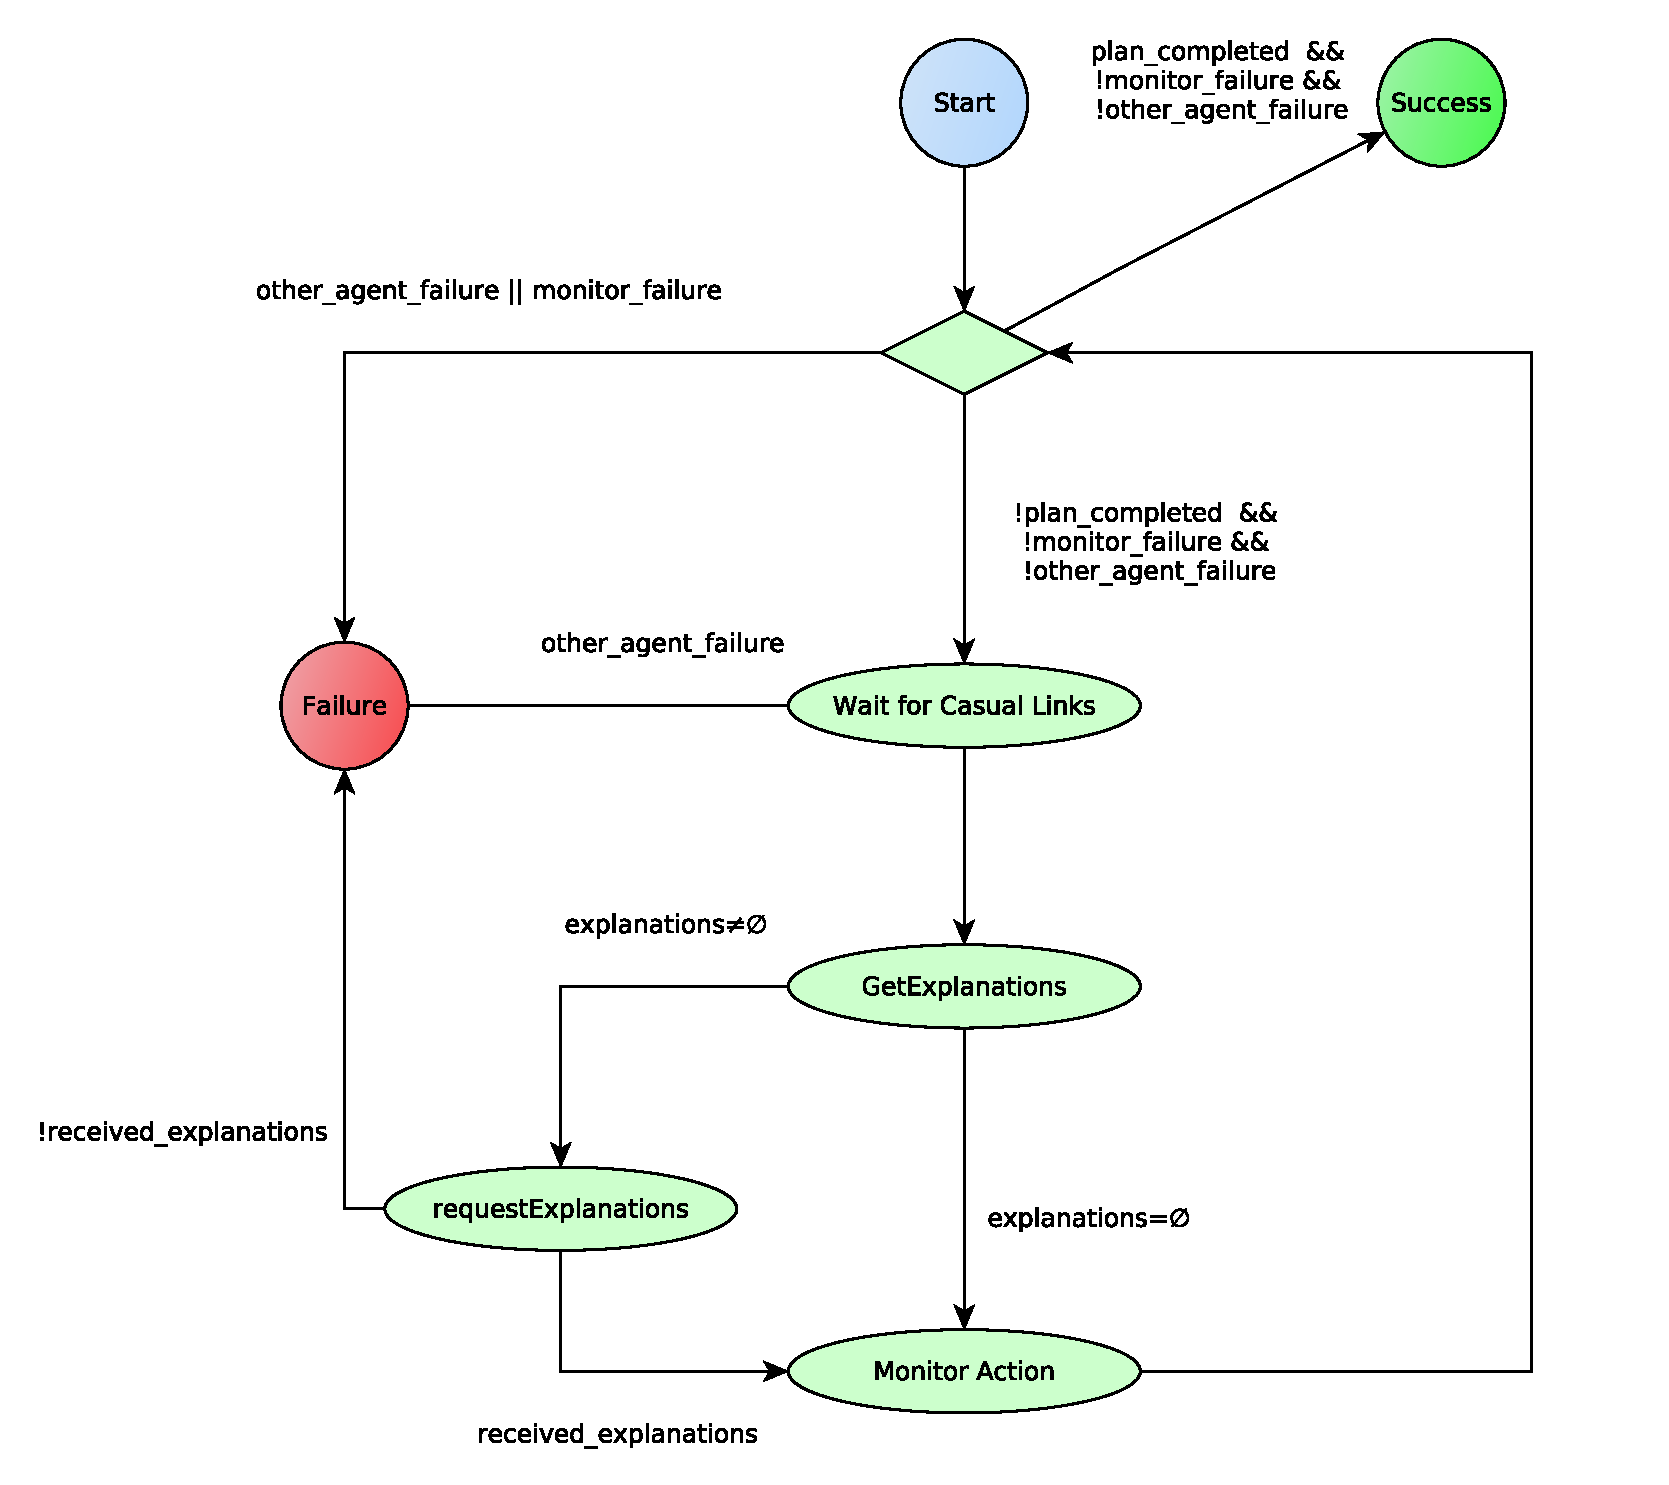
\includegraphics[scale=0.5]{img/plan_management/manage_plan_leader_humans.pdf}
 \caption[The human parallel plan management algorithm]{The human parallel plan management algorithm used when the current modality is \textit{robot leader}. The symbols used are the same as in the previous image, figure \ref{fig:plan_management-manage_plan_leader_control_block}.}
 \label{fig:plan_management-manage_plan_leader_humans}
 \end{figure}


\subsubsection{Human Knowledge and Warnings}
Maintaining human knowledge is done exactly in the same way as the sequential plan manager. The robot will issue a warning to a human when he commits a mistake.

\subsubsection{Replanning}
When the plan manager reports a failure, the system needs to look for a new plan. If possible, we would like to create a plan which contains the same high-level task allocation. Sometimes, when the Plan Manager fails, there is no need to completely change the plan. Instead, it might be sufficient to repair only a part of it. For example, we can imagine a scenario where a human might execute task $t_1$ using resource $r_1$ or $r_2$. Perhaps the robot computed a plan where the human will use resource $r_1$, while itself will use $r_2$ to achieve another task.

If the human does not follow this plan, and uses $r_2$ to compute its task,  it might be faster to just repair the plan, looking for a solution where the task allocation is the same, but the robot uses $r_1$ instead to achieve its task. This way, we avoid starting a new explanation\textbackslash negotiation phase, which could look useless and not natural to the human collaborator.

%  We deal with this issue in different ways in HATP and HAPP.

In HATP, we introduce a new cost rule. When presenting a plan, we record which nodes have been presented and assigned to each agent. While planning, we penalize plans with a different task allocation. This way, the planner will prefer to use the same task allocation, but will change it if needed, for example because, using the previous task allocation, the goal is no longer achievable.

%In HAPP, we can just perform a partial replan, by interrogating the currently active MMODP.  
